%!TEX root = ../thesis.tex

\chapter{Implementierung und Evaluation} % (fold)
\label{cha:implementierung_und_evaluation}

\section{Verwendete Bibliotheken} % (fold)
\label{sec:verwendete_bibliotheken}

\subsection{RDF2Go} % (fold)
\label{sub:rdf2go}

% subsection rdf2go (end)



% section verwendete_bibliotheken (end)

\section{Implementierung der Connectoren} % (fold)
\label{sec:implementierung_der_connectoren}

Das muss rein:
\begin{itemize}
    \item Mapping nach SIOC
    \item Zugriff über die API
    \item Probleme bei der Implementierung
\end{itemize}

Innerhalb der Mappingbeschreibungen zwischen den Format der einzelnen SOC und SIOC werden zur besseren Übersicht und einfacheren Lesbarkeit Platzhalt für einige URIs benutzt. Welche Platzhalten dies sind und für welche URI sie stehen ist aus Tabelle \ref{tbl:platzhalter_fuer_sioc_mapping} zu entnehmen. Für die einzelnen SOC werden noch einmal gesonderte Platzhalter definiert, diese werden aber gesondert in den einzelnen Abschnitten beschrieben. 

\begin{table}[h]
    \centering
    \caption{Allgemeine Platzhalter und deren Beschreibung für das Mapping nach SIOC}
    \begin{tabular}{l|p{11cm}}
        \textbf{Platzhalter} & \textbf{Bedeutung} \\ 
        \hline
        \texttt{\{serviceUri\}} & URI für einen Service \\
        \texttt{\{userAccountUri\}} & URI für einen UserAccount \\
        \texttt{\{siteUri\}} & URI für eine Site \\
        \texttt{\{forumUri\}} & URI für ein Forum \\
        \texttt{\{threadUri\}} & URI für ein Thread \\
        \texttt{\{postUri\}} & URI für ein Post \\
        \texttt{\{rootUri\}} & Die WurzelUri einer SOC. Für Facebook wäre dies zum Beispiel \texttt{https://www.facebook.com}
    \end{tabular}
    \label{tbl:platzhalter_fuer_sioc_mapping}
\end{table}

\subsection{Moodle} % (fold)
\label{sub:moodle_connector}

\begin{itemize}
    \item Eingebaute REST Schnittstelle, aber kein Lesen von Beiträgen
    \item WebService Plugin MoodleWS (REST oder SOAP)
    \begin{itemize}
        \item https://github.com/patrickpollet/moodlews
        \item ClientAPI existieren von selber Autor
        \item REST defekt, kein schreiben von Beiträgen möglich
        \item SOAP funktioniert mehr oder weniger
        \item Verschluckt Fehlermeldungen
        \item kein lesen einzelner Posts/Threads/Foren
        \item SOAP ClientAPI neu generieren, weil vorhandene nicht mit 2.4 funktioniert.
        \item Username/Password + Session Token/Id
        \item “Use an auto generated wsdl” -> No
        \item schreiben von neuen Beitrag direkt in thread nur als Antwort auf ersten Beitrag möglich
        \item Rückgabe aller Beiträge in einem Objekt
    \end{itemize}
\end{itemize}

\subsubsection{SIOC Mapping} % (fold)
\label{ssub:moodle_sioc_mapping}

\subsubsection{API} % (fold)
\label{ssub:moolde_api}

\subsubsection{Herausforderungen} % (fold)
\label{ssub:moodle_herausforderungen}

% subsubsection moodle_herausforderungen (end)

% subsubsection moodle_api (end)

% subsubsection moodle_sioc_mapping (end)

% subsection moodle_connector (end)

\subsection{Facebook} % (fold)
\label{sub:facebook_connector}

\begin{itemize}
    \item REST API + JSON
    \item keine offizielle Java API für Desktop -> Web + Mobile only
    \item GraphAPI, Facebook Query Language
    \item OAuth 2.x
    \begin{itemize}
        \item kein Refreshtoke
        \item Token Haltbarkeit 2h (2 Monate, wen extended)
        \item token nur über webbrowser
    \end{itemize}
    \item RestFB alternative Java API für die REST Schnittstelle der GraphAPI
    \item Typ der zurückgelieferten Daten nicht anhand der URI erkennbar, häufig erst durch Angabe von \emph{metadata=1}
    \item beim herunterladen einzelner Posts nicht immer erkennbar wo sie geschrieben wurden
\end{itemize}

\subsubsection{SIOC Mapping} % (fold)
\label{ssub:facebook_sioc_mapping}

\subsubsection{API} % (fold)
\label{ssub:facebook_api}

\subsubsection{Herausforderungen} % (fold)
\label{ssub:facebook_herausforderungen}

% subsubsection facebook_herausforderungen (end)

% subsubsection facebook_api (end)

% subsubsection facebook_sioc_mapping (end)

% subsection facebook_connector (end)

\subsection{Google+} % (fold)
\label{sub:google_plus_connector}

\begin{itemize}
    \item Einfach REST API + JSON
    \item OAuth
    \begin{itemize}
        \item Refreshtoken (token laufen quasi nie ab)
        \item holen von token ohne webbrowser möglich
    \end{itemize}
    \item Objekte aufgebaut aus Actor (wer machte was), Verb(wie machte er es), Object (wtas machte er) + Metadata
    \item verschieden Sprachen + Plattformen
    \item lesen nur von öffentlichen Beiträgen
    \item kein Schreiben von Beiträgen
\end{itemize}

\subsubsection{SIOC Mapping} % (fold)
\label{ssub:google_plus_sioc_mapping}

\subsubsection{API} % (fold)
\label{ssub:google_plus_api}

\subsubsection{Herausforderungen} % (fold)
\label{ssub:google_plus_herausforderungen}

% subsubsection google_plus_herausforderungen (end)

% subsubsection google_plus_api (end)

% subsubsection google_plus_sioc_mapping (end)

% subsection google_plus_connector (end)

\subsection{Youtube } % (fold)
\label{sub:youtube_connector}

\begin{itemize}
    \item Aktueller Umbau der API (ähnlich google+) v3
    \begin{itemize}
        \item keine lesen von kommentaren
        \item kein schreiben
    \end{itemize}
    \item alte GData Feed API v2 basiert auf RSS + Youtube Erweiterung
    \item Mapping teilweise durch basis auf RSS einfach, manchmal auch nicht
    \item Wichtigen Metadaten nur implizit vorhanden (comment id in uri aber nicht in datenformat)
\end{itemize}

\subsubsection{SIOC Mapping} % (fold)
\label{ssub:youtube_sioc_mapping}

\subsubsection{API} % (fold)
\label{ssub:youtube_api}

\subsubsection{Herausforderungen} % (fold)
\label{ssub:youtube_herausforderungen}

% subsubsection youtube_herausforderungen (end)

% subsubsection youtube_api (end)

% subsubsection youtube_sioc_mapping (end)

% subsection youtube_connector (end)

\subsection{Canvas} % (fold)
\label{sub:canvas_connector}

\begin{itemize}
    \item relativ neues LMS
    \item super Bedienung
    \item super REST API
    \item keine Java API
    \item rudimentäre Eigenentwicklung einer Java API, Funktionsweise ähnlich  G+
    \item viel API Funktionen wohl nicht extern nutzbar (UserProfil lesen, vll. Falsche Berechtigung -> test nötig)
\end{itemize}

\subsubsection{Canvas REST-API} % (fold)
\label{ssub:canvas_api}

Der öffentliche Zugriff auf die Daten von der Lernplattform Canvas basiert auf einer REST-API und OAuth 2.0 zur Autorisierung der Zugriffe. Die Adresse, über die auf die API zugegriffen werden kann, besteht aus der URI für die verwendete Canvas Instanz (\texttt{\{rootUri\}}) und gefolgt von dem Pfad \enquote{/api/v1}. Für die Demo Instanz von Instructre würde dies der URI \texttt{https://canvas.instructure.com/api/v1} entsprechen. An diese können dann weitere Pfade für den Zugriff auf die einzelnen Ressourcen angehängt werden. Zur Autorisierung wird von OAuth nur der Accesstoken benötigt, der bei der REST-Abfrage als HTTP Authorization Header mitgeschickt wird. Listing \ref{lst:canvas_authorization_header} zeigt eine eine Beispielanfrage und Angabe des Accesstokens mit dem Programm \emph{curl}\footnote{\url{http://curl.haxx.se/}}. Der Platzhalter \texttt{\{accessToken\}} muss dann natürlich erst durch einen validen Accesstoken ersetzt werden. Diesen kann jeder Benutzter in seinem Canvas Profil unter \enquote{Settings} und im Abschnitt \enquote{Approved Integrations} selbst erstellen. Die Angabe von ClientId und ClientSecret von OAuth 2.0 sind nicht nötig.

\begin{lstlisting}[
    caption={Canvas Authorization Header}\label{lst:canvas_authorization_header},
    captionpos=t]
curl -H "Authorization: Bearer {accessToken}" https://canvas.instructure.com/api/v1/courses
\end{lstlisting}

Als Datenformat für die zurückgelieferten Daten wird von der Canvas API auf JSON gesetzt. Für die Verwendung von POST und PUT Operationen zum Schreiben nach Canvas können die Daten entweder nach dem HTML Form Encoding\footnote{\url{http://www.w3.org/TR/html4/interact/forms.html\#h-17.13.4}} Standard oder ebenfalls in JSON angegeben werden. 

Da einige Anfragen eine Liste von Ergebnissen zurückliefern und diese möglicher Weise lang werden können, teilt die Canvas API diese Listen auf mehrere Seiten auf, die jede einzeln abgefragt werden müssen. Für jede Seite schickt die Canvas API mehrere URIs als HTTP Link Header\footnote{\url{http://www.w3.org/Protocols/9707-link-header.html}} der Antwort mit. Diese URIs erhalten zusätzlich noch ein Attribut \texttt{rel}, das beschreibt in welcher Relation die URI zu dieser Seite steht.  Als Wert für diese Relation können \enquote{current} für eine URI auf die aktuelle, \enquote{next} auf die nächste, \enquote{prev} auf die vorherige, \enquote{first} auf die erste und \enquote{last} für eine URI auf die letzte Seite vorkommen. Um also die nächste Seite vom Ergebnis zu bekommen, muss eine neue REST-Anfrage mit der Relation \enquote{next} ausgeführt werden. Fehlt eine URI mit dieser Relation, ist das die letzte Seite erreicht. 

% subsubsection canvas_api (end)

\subsubsection{CanvasLMS4J} % (fold)
\label{ssub:canvaslms4j}

Ein Problem mit der API von Canvas war es, dass es zwar eine gute REST Anbindung gab, aber noch keine Bibliothek um sie mit der Programmiersprache Java anzusprechen. Es musste also erst eine eigne Java API dazu entwickelt werden, die den Namen \emph{CanvasLMS4J} (Kurzform für \enquote{Canvas LMS API für Java}) bekam. 

Anhand der für die REST API verwendeten URIs ist auffällig, dass die einzelnen Bestandteile aufeinander aufbauen. Zum Beispiel ist der Ablauf für den REST-Zugriff auf DiscussionTopics in Gruppen und Kursen der gleiche, nur die verwendete URI unterscheidet sich. Aus diesem Grund wurden die einzelnen Ressource (Course, Groupe, DiscussionTopic, Entries, ...) als einzelne Endpunkte implementiert die sich von der Klasse \texttt{IEnpoint} ableiten. Jeder Endpunkt kann einen Eltern-Endpunkt haben, wobei sich die endgültige URI für die REST-Abfrage aus dem Pfad des Eltern-Endpunktes und dem des aktuellen Endpunktes zusammensetzt. Zur Verdeutlichung sei hier die URI \texttt{https:\{canvasUri\}/api/v1/courses/1/discussion\_topics} als Demonstration genannt. Sie besteht aus den statischen Teil \texttt{https:\{canvasUri\}/api/v1/} der den Ort für die verwendete Canvas Instanz angibt. Darauf folgt ein Kurs als erster Endpunkt mit der Kurs-ID \enquote{1}. Für diesen Kurs sollen nun alle Diskussionen abgefragt werden. Dies geschieht durch die Angabe des zweiten Endpunktes \texttt{/discussion\_topics}. \enquote{/courses/1} bildet hier also den Eltern-Endpunkt von \texttt{/discussion\_topics}. Sollen aber nun alle Diskussionen in einer Gruppe abgefragt werden, reicht es aus den Kurs-Endpunkt durch einen Gruppen-Endpunkt auszutauschen.

\begin{figure}[ht]
    \centering
    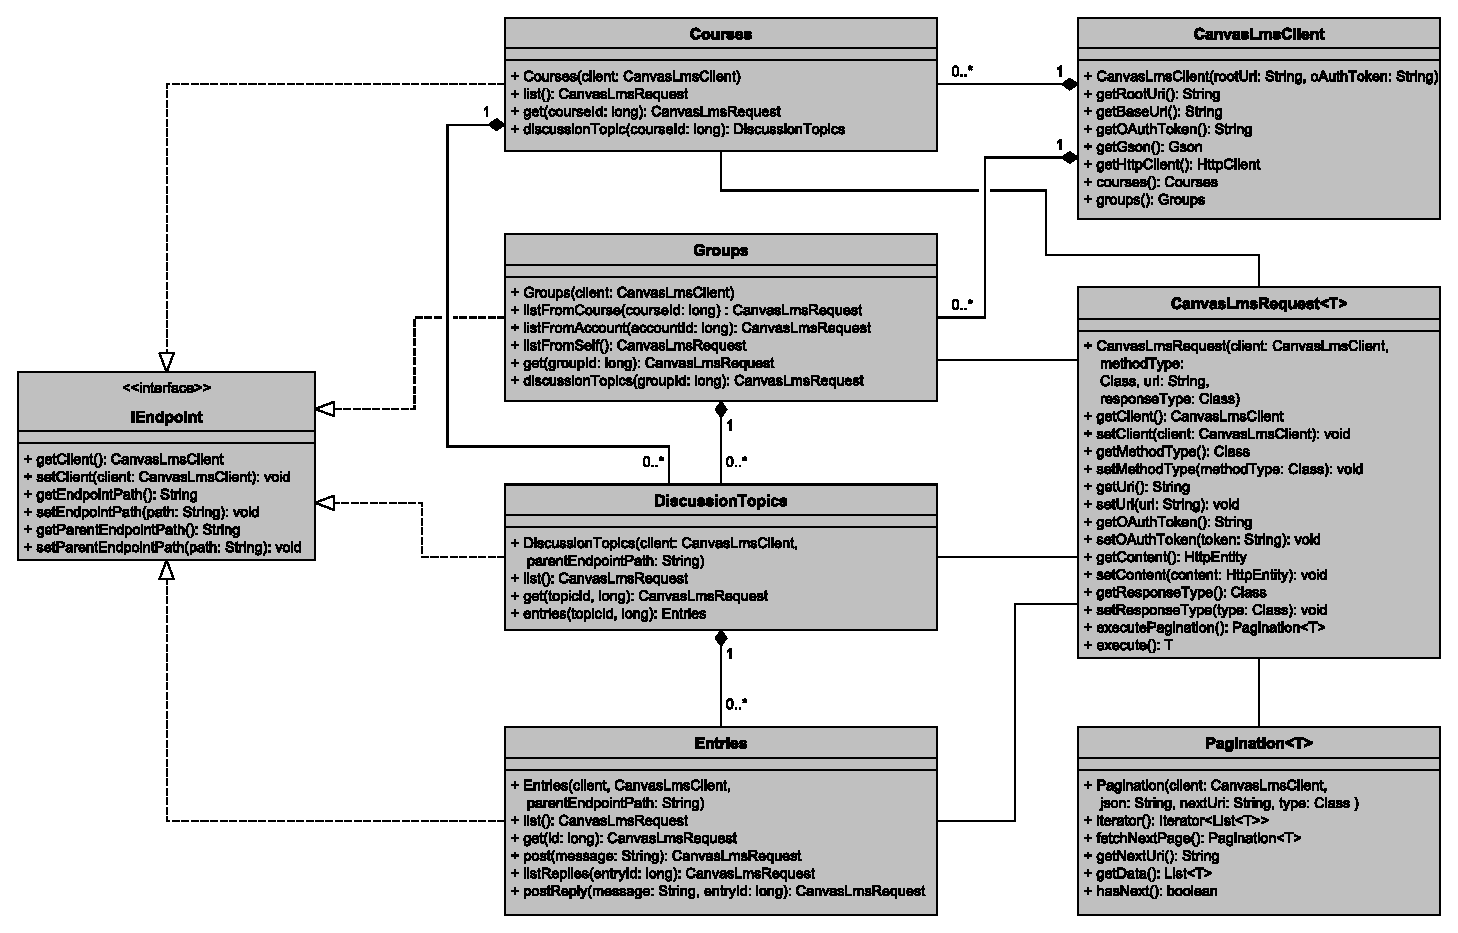
\includegraphics[
        width=\textwidth,
        keepaspectratio=true,]
    {assets/images/canvaslms4j_uml_classdiagramm}
    \caption{UML Klassendiagramm von CanvasLMS4J}
    \label{fig:canvaslms4j_uml_classdiagram}
\end{figure} 

Ausgangspunkt für CanvasLMS4J ist die Klasse \texttt{CanvasLmsClient} (siehe Abbildung \ref{fig:canvaslms4j_uml_classdiagram}). Über sie werden alle Endpunkte verwaltet die keinen Eltern-Endpunkt besitzen. Bei der Erzeugung eines Objektes dieser Klasse, werden ihr die URI zur verwendenden Canvas Instanz und der AccessToken des Benutzerkontos übergeben. Im aktuellen Stadium können von einem Client aus nur Endpunkte für Kurse oder Gruppe erstellt werden.

Endpunkte können dann über die Klasse \texttt{CanvasLmsRequest} REST-Anfragen an die Canvas API stellen. Hierzu verwendet CanvasLMS4J die \emph{HttpClient}\footnote{\url{http://hc.apache.org/httpclient-3.x/}} Bibliothek von Apache mit die einzelnen HTTP-Operationen ausgeführt werden. Um die im JSON-Format zurück gelieferten Antworten der Canvas API in Java verwenden zu können, wir auf die Funktionen der von Google entwickelten \emph{Gson}\footnote{\url{https://code.google.com/p/google-gson/}} Bibliothek zurück gegriffen. Sie erlaubt es Java Objekte in das JSON-Format zu konvertieren und genauso aus Daten in JSON ein Java Objekt zu machen. Dadurch verringert sich der Aufwand für das Verarbeiten der Daten von Canvas auf das Erstellen der entsprechenden Java Klassen. CanvasLmsRequest können mit zwei verschiedenen Methoden ausgeführt werden. Die erste \texttt{execute()} wird dazu verwendet, wenn die REST-Abfrage nur die Rückgabe eines Objektes zu Folge hat. Also zum Beispiel, wenn nur die Daten eines bestimmten Kurses abgefragt werden soll. Die zweite Methode ist \texttt{executePagination}. Diese Methode dient für Abfragen die eine in Seiten aufgeteilte Liste von Ergebnissen zurückliefert und gibt für eine einfache Handhabbarkeit ein Objekt der Klasse \texttt{Pagination} zurück. 

Die Klasse Pagination ist nach dem Iterator Muster aufgebaut und liefert vom kompletten Ergebnis bei jedem Iterationsschritt eine Seite zurück. Diese Seite enthält dann je eine Teilliste der angefragten Objekten. Ist eine Seite fertig ausgelesen, holt Pagination über eine vorgegeben REST Abfrage die nächste Seite. Dies geschieht solange bis keine Seiten mehr geladen werden können oder das Programm das Lesen abbricht.

\begin{lstlisting}[
    caption={CanvasLMS4J Beispielprogramm}\label{lst:canvaslms4j_beispiel},
    captionpos=t]
CanvasLmsClient client = new CanvasLmsClient(
                "https://canvas.instructure.com",
                "7~LUpV7B3lJY...");

Pagination<DiscussionTopic> discussionPages = client.courses()
    .discussionTopics( 798152 )
    .list()
    .executePagination();


for ( List<DiscussionTopic> discussions : discussionPages ) {
    for ( DiscussionTopic discussion : discussions ) {
        System.out.println( discussion );
    }
}

\end{lstlisting}

In Listing \ref{lst:canvaslms4j_beispiel} ist ein Beispiel für die Anwendung der CanvasLMS4J API zu sehen. In den ersten drei Zeilen wird eine neuer CanvasLmsClient für die Canvas Instanz auf \texttt{https://canvas.instructure.com} und einem AccessToken erstellt. Als nächstes soll für einen Kurs mit der ID \enquote{798152} alle Diskussionen aufgelistet werden. Mit dem Aufruf der Methode \texttt{courses()} des Clients wir der Endpunkt für die Kurse und von diesem aus der Endpunkt für die Diskussionen im Kurs \enquote{798152} über die Methode \texttt{.discussionTopics( 798152 )}. In der siebten Zeile wird die Art der Abfrage genauer festgelegt. Da eine Liste alle Diskussionen gesucht ist, wird die Methode \texttt{list()} aufgerufen die ein CanvasLmsRequest Objekt für die gewünschte Abfrage erstellt. Da die Antwort aus mehrere Objekten mit der Beschreibung der einzelnen Diskussionen besteht, wird die Anfrage in Zeile Acht mit der Methode \texttt{executePagination()} ausgeführt. Die einzelnen Seiten des Ergebnisses werden dann in der elften Zeile mit einer For-Schleife durchlaufen. Das nachladen der Seiten erfolgt dabei automatisch durch die Pagination Klasse. Jede Seite besteht nun aus einer Liste mit den Beschreibung der Diskussionen in einem \texttt{DiskussionTopic} Objekt, welche dann wieder in einer weiteren Schleife ausgegeben werden.

% subsubsection canvaslms4j (end)

\subsubsection{Canvas Mapping nach SIOC} % (fold)
\label{ssub:canvas_sioc_mapping}

\begin{table}[h]
    \centering
    \caption{Format der URIs für Canvas}
    \begin{tabular}{l|p{11cm}}
        \textbf{URI Platzhalter} & URI-Format \\ 
        \hline
        \texttt{\{serviceUri\}} & 
        \texttt{\{rootUri\}/api/v1} \\

        \texttt{\{userAccountUri\}} & 
        \texttt{\{rootUri\}/about/\{userId\}} \\

        \texttt{\{siteUri\}} & 
        \texttt{\{rootUri\}} \\

        \texttt{\{forumUri\}} & 
        \texttt{\{rootUri\}/courses/\{courseId\}},
        \texttt{\{rootUri\}/groups/\{groupId\}} \\

        \texttt{\{threadUri\}} & 
        \texttt{\{forumUri\}/discussion\_topics/\{topicId\}} \\

        \texttt{\{postUri\}} & 
        \texttt{\{threadUri\}/entries/\{entryId\}},
        \texttt{\{threadUri\}\#discussion\_topic} \\
    \end{tabular}
    \label{tbl:canvas_uri_platzhalter}
\end{table}

% subsubsection canvas_sioc_mapping (end)

% subsection canvas_connector (end)

% section implementierung_einiger_connectoren (end)

\section{Evaluation} % (fold)
\label{sec:evaluation}

% section evaluation (end)

% chapter implementierung_und_evaluation (end)